\documentclass[twoside]{book}

% Packages required by doxygen
\usepackage{fixltx2e}
\usepackage{calc}
\usepackage{doxygen}
\usepackage[export]{adjustbox} % also loads graphicx
\usepackage{graphicx}
\usepackage[utf8]{inputenc}
\usepackage{makeidx}
\usepackage{multicol}
\usepackage{multirow}
\PassOptionsToPackage{warn}{textcomp}
\usepackage{textcomp}
\usepackage[nointegrals]{wasysym}
\usepackage[table]{xcolor}

% Font selection
\usepackage[T1]{fontenc}
\usepackage[scaled=.90]{helvet}
\usepackage{courier}
\usepackage{amssymb}
\usepackage{sectsty}
\renewcommand{\familydefault}{\sfdefault}
\allsectionsfont{%
  \fontseries{bc}\selectfont%
  \color{darkgray}%
}
\renewcommand{\DoxyLabelFont}{%
  \fontseries{bc}\selectfont%
  \color{darkgray}%
}
\newcommand{\+}{\discretionary{\mbox{\scriptsize$\hookleftarrow$}}{}{}}

% Page & text layout
\usepackage{geometry}
\geometry{%
  a4paper,%
  top=2.5cm,%
  bottom=2.5cm,%
  left=2.5cm,%
  right=2.5cm%
}
\tolerance=750
\hfuzz=15pt
\hbadness=750
\setlength{\emergencystretch}{15pt}
\setlength{\parindent}{0cm}
\setlength{\parskip}{3ex plus 2ex minus 2ex}
\makeatletter
\renewcommand{\paragraph}{%
  \@startsection{paragraph}{4}{0ex}{-1.0ex}{1.0ex}{%
    \normalfont\normalsize\bfseries\SS@parafont%
  }%
}
\renewcommand{\subparagraph}{%
  \@startsection{subparagraph}{5}{0ex}{-1.0ex}{1.0ex}{%
    \normalfont\normalsize\bfseries\SS@subparafont%
  }%
}
\makeatother

% Headers & footers
\usepackage{fancyhdr}
\pagestyle{fancyplain}
\fancyhead[LE]{\fancyplain{}{\bfseries\thepage}}
\fancyhead[CE]{\fancyplain{}{}}
\fancyhead[RE]{\fancyplain{}{\bfseries\leftmark}}
\fancyhead[LO]{\fancyplain{}{\bfseries\rightmark}}
\fancyhead[CO]{\fancyplain{}{}}
\fancyhead[RO]{\fancyplain{}{\bfseries\thepage}}
\fancyfoot[LE]{\fancyplain{}{}}
\fancyfoot[CE]{\fancyplain{}{}}
\fancyfoot[RE]{\fancyplain{}{\bfseries\scriptsize Generated by Doxygen }}
\fancyfoot[LO]{\fancyplain{}{\bfseries\scriptsize Generated by Doxygen }}
\fancyfoot[CO]{\fancyplain{}{}}
\fancyfoot[RO]{\fancyplain{}{}}
\renewcommand{\footrulewidth}{0.4pt}
\renewcommand{\chaptermark}[1]{%
  \markboth{#1}{}%
}
\renewcommand{\sectionmark}[1]{%
  \markright{\thesection\ #1}%
}

% Indices & bibliography
\usepackage{natbib}
\usepackage[titles]{tocloft}
\setcounter{tocdepth}{3}
\setcounter{secnumdepth}{5}
\makeindex

% Hyperlinks (required, but should be loaded last)
\usepackage{ifpdf}
\ifpdf
  \usepackage[pdftex,pagebackref=true]{hyperref}
\else
  \usepackage[ps2pdf,pagebackref=true]{hyperref}
\fi
\hypersetup{%
  colorlinks=true,%
  linkcolor=blue,%
  citecolor=blue,%
  unicode%
}

% Custom commands
\newcommand{\clearemptydoublepage}{%
  \newpage{\pagestyle{empty}\cleardoublepage}%
}

\usepackage{caption}
\captionsetup{labelsep=space,justification=centering,font={bf},singlelinecheck=off,skip=4pt,position=top}

%===== C O N T E N T S =====

\begin{document}

% Titlepage & ToC
\hypersetup{pageanchor=false,
             bookmarksnumbered=true,
             pdfencoding=unicode
            }
\pagenumbering{alph}
\begin{titlepage}
\vspace*{7cm}
\begin{center}%
{\Large emotions }\\
\vspace*{1cm}
{\large Generated by Doxygen 1.8.13}\\
\end{center}
\end{titlepage}
\clearemptydoublepage
\pagenumbering{roman}
\tableofcontents
\clearemptydoublepage
\pagenumbering{arabic}
\hypersetup{pageanchor=true}

%--- Begin generated contents ---
\chapter{Hierarchical Index}
\section{Class Hierarchy}
This inheritance list is sorted roughly, but not completely, alphabetically\+:\begin{DoxyCompactList}
\item \contentsline{section}{Emotions\+Configuration}{\pageref{class_emotions_configuration}}{}
\item \contentsline{section}{Emotions\+Data}{\pageref{class_emotions_data}}{}
\item \contentsline{section}{Emotions\+Tracker}{\pageref{class_emotions_tracker}}{}
\item Handler\begin{DoxyCompactList}
\item \contentsline{section}{Emotions\+Handler}{\pageref{class_emotions_handler}}{}
\end{DoxyCompactList}
\end{DoxyCompactList}

\chapter{Class Index}
\section{Class List}
Here are the classes, structs, unions and interfaces with brief descriptions\+:\begin{DoxyCompactList}
\item\contentsline{section}{\hyperlink{class_emotions_configuration}{Emotions\+Configuration} \\*Class for providing iterface to configure Emotions Tracker behaviors }{\pageref{class_emotions_configuration}}{}
\item\contentsline{section}{\hyperlink{class_emotions_data}{Emotions\+Data} \\*Class for providing iterface to collected emotions data }{\pageref{class_emotions_data}}{}
\item\contentsline{section}{\hyperlink{class_emotions_handler}{Emotions\+Handler} \\*Class for providing the camera event handler }{\pageref{class_emotions_handler}}{}
\item\contentsline{section}{\hyperlink{class_emotions_tracker}{Emotions\+Tracker} \\*Class for providing the driver to process data from camera }{\pageref{class_emotions_tracker}}{}
\end{DoxyCompactList}

\chapter{Class Documentation}
\hypertarget{class_emotions_configuration}{}\section{Emotions\+Configuration Class Reference}
\label{class_emotions_configuration}\index{Emotions\+Configuration@{Emotions\+Configuration}}


Class for providing iterface to configure Emotions Tracker behaviors  




{\ttfamily \#include $<$emotracker.\+h$>$}

\subsection*{Public Member Functions}
\begin{DoxyCompactItemize}
\item 
void \hyperlink{class_emotions_configuration_a59ff9feb080a20721a2ba714fc9f40dc}{set\+Stream\+Filename} (pxc\+C\+H\+AR $\ast$stream\+Filename)
\item 
void \hyperlink{class_emotions_configuration_a4645e007a7b2a9d9c52f020530b401fb}{set\+Calibration\+Filename} (pxc\+C\+H\+AR $\ast$calib\+Filename)
\item 
void \hyperlink{class_emotions_configuration_a7b8cdc24a83960cef6579cc4ce454709}{set\+Emotions\+Filename} (pxc\+C\+H\+AR $\ast$emo\+Filename)
\item 
void \hyperlink{class_emotions_configuration_afa77034583065b49e1ed9bdfe4ad1d77}{set\+Person\+Tracking} (pxc\+Bool person\+Tracking)
\item 
void \hyperlink{class_emotions_configuration_a712005bb21d3745664a9ff1c23466fc3}{set\+Add\+Gaze\+Point} (pxc\+Bool add\+Gaze\+Point)
\item 
void \hyperlink{class_emotions_configuration_a6d50830265d85761f5dd0abfa12d5fcb}{set\+Recording\+Landmark} (pxc\+Bool recording\+Landmark)
\item 
void \hyperlink{class_emotions_configuration_af52d273380cd9392a2ff104b774b5da9}{set\+Recording\+Gaze} (pxc\+Bool recording\+Gaze)
\item 
void \hyperlink{class_emotions_configuration_a1eb27ec836c4151d78a826a50566e3a3}{set\+Use\+Person\+Tracking\+Module\+Emotions} (pxc\+Bool use\+Person\+Tracking\+Module\+Emotions)
\end{DoxyCompactItemize}
\subsection*{Public Attributes}
\begin{DoxyCompactItemize}
\item 
\mbox{\Hypertarget{class_emotions_configuration_abd2c50caf6290933d5044e49b218f207}\label{class_emotions_configuration_abd2c50caf6290933d5044e49b218f207}} 
pxc\+C\+H\+AR $\ast$ {\bfseries calib\+Filename} = L\char`\"{}calib.\+bin\char`\"{}
\item 
\mbox{\Hypertarget{class_emotions_configuration_a2cdaff812ec953152f9648448859f44e}\label{class_emotions_configuration_a2cdaff812ec953152f9648448859f44e}} 
pxc\+C\+H\+AR $\ast$ {\bfseries stream\+Filename} = L\char`\"{}1.rssdk\char`\"{}
\item 
\mbox{\Hypertarget{class_emotions_configuration_a0acd66cdfc61dde2654762c5b43f9c89}\label{class_emotions_configuration_a0acd66cdfc61dde2654762c5b43f9c89}} 
pxc\+C\+H\+AR $\ast$ {\bfseries emo\+Filename} = L\char`\"{}1.ttml\char`\"{}
\item 
\mbox{\Hypertarget{class_emotions_configuration_ab1df9d7d072e50194dc3d85b38c6d6cb}\label{class_emotions_configuration_ab1df9d7d072e50194dc3d85b38c6d6cb}} 
pxc\+Bool {\bfseries person\+Tracking} = true
\item 
\mbox{\Hypertarget{class_emotions_configuration_a5e1ccf5105dd5bfed0fc021c4c8a32d4}\label{class_emotions_configuration_a5e1ccf5105dd5bfed0fc021c4c8a32d4}} 
pxc\+Bool {\bfseries add\+Gaze\+Point} = true
\item 
\mbox{\Hypertarget{class_emotions_configuration_a88d1643658f047c84d85f1a786762a3f}\label{class_emotions_configuration_a88d1643658f047c84d85f1a786762a3f}} 
pxc\+Bool {\bfseries recording\+Landmark} = true
\item 
\mbox{\Hypertarget{class_emotions_configuration_a127e56275ce6a1326e85a35ac981a211}\label{class_emotions_configuration_a127e56275ce6a1326e85a35ac981a211}} 
pxc\+Bool {\bfseries recording\+Gaze} = true
\item 
\mbox{\Hypertarget{class_emotions_configuration_a59bf0871027ddc0702774b9d3e24ec7b}\label{class_emotions_configuration_a59bf0871027ddc0702774b9d3e24ec7b}} 
pxc\+Bool {\bfseries use\+Person\+Tracking\+Module\+Emotions} = false
\end{DoxyCompactItemize}


\subsection{Detailed Description}
Class for providing iterface to configure Emotions Tracker behaviors 

\subsection{Member Function Documentation}
\mbox{\Hypertarget{class_emotions_configuration_a712005bb21d3745664a9ff1c23466fc3}\label{class_emotions_configuration_a712005bb21d3745664a9ff1c23466fc3}} 
\index{Emotions\+Configuration@{Emotions\+Configuration}!set\+Add\+Gaze\+Point@{set\+Add\+Gaze\+Point}}
\index{set\+Add\+Gaze\+Point@{set\+Add\+Gaze\+Point}!Emotions\+Configuration@{Emotions\+Configuration}}
\subsubsection{\texorpdfstring{set\+Add\+Gaze\+Point()}{setAddGazePoint()}}
{\footnotesize\ttfamily void Emotions\+Configuration\+::set\+Add\+Gaze\+Point (\begin{DoxyParamCaption}\item[{pxc\+Bool}]{add\+Gaze\+Point }\end{DoxyParamCaption})}


\begin{DoxyParams}{Parameters}
{\em add\+Gaze\+Point} & Provides ability to write gaze point to the subtitles in output ttml file. By default is {\bfseries true}\\
\hline
\end{DoxyParams}
\mbox{\Hypertarget{class_emotions_configuration_a4645e007a7b2a9d9c52f020530b401fb}\label{class_emotions_configuration_a4645e007a7b2a9d9c52f020530b401fb}} 
\index{Emotions\+Configuration@{Emotions\+Configuration}!set\+Calibration\+Filename@{set\+Calibration\+Filename}}
\index{set\+Calibration\+Filename@{set\+Calibration\+Filename}!Emotions\+Configuration@{Emotions\+Configuration}}
\subsubsection{\texorpdfstring{set\+Calibration\+Filename()}{setCalibrationFilename()}}
{\footnotesize\ttfamily void Emotions\+Configuration\+::set\+Calibration\+Filename (\begin{DoxyParamCaption}\item[{pxc\+C\+H\+AR $\ast$}]{calib\+Filename }\end{DoxyParamCaption})}


\begin{DoxyParams}{Parameters}
{\em calib\+Filename} & Provides ability to setup the input filename with gaze calibration data in rssdk format. By default used {\bfseries calib.\+bin}\\
\hline
\end{DoxyParams}
\mbox{\Hypertarget{class_emotions_configuration_a7b8cdc24a83960cef6579cc4ce454709}\label{class_emotions_configuration_a7b8cdc24a83960cef6579cc4ce454709}} 
\index{Emotions\+Configuration@{Emotions\+Configuration}!set\+Emotions\+Filename@{set\+Emotions\+Filename}}
\index{set\+Emotions\+Filename@{set\+Emotions\+Filename}!Emotions\+Configuration@{Emotions\+Configuration}}
\subsubsection{\texorpdfstring{set\+Emotions\+Filename()}{setEmotionsFilename()}}
{\footnotesize\ttfamily void Emotions\+Configuration\+::set\+Emotions\+Filename (\begin{DoxyParamCaption}\item[{pxc\+C\+H\+AR $\ast$}]{emo\+Filename }\end{DoxyParamCaption})}


\begin{DoxyParams}{Parameters}
{\em emo\+Filename} & Provides ability to setup the output filename with collected emotions data in ttml format. By default used {\bfseries 1.\+ttml}\\
\hline
\end{DoxyParams}
\mbox{\Hypertarget{class_emotions_configuration_afa77034583065b49e1ed9bdfe4ad1d77}\label{class_emotions_configuration_afa77034583065b49e1ed9bdfe4ad1d77}} 
\index{Emotions\+Configuration@{Emotions\+Configuration}!set\+Person\+Tracking@{set\+Person\+Tracking}}
\index{set\+Person\+Tracking@{set\+Person\+Tracking}!Emotions\+Configuration@{Emotions\+Configuration}}
\subsubsection{\texorpdfstring{set\+Person\+Tracking()}{setPersonTracking()}}
{\footnotesize\ttfamily void Emotions\+Configuration\+::set\+Person\+Tracking (\begin{DoxyParamCaption}\item[{pxc\+Bool}]{person\+Tracking }\end{DoxyParamCaption})}


\begin{DoxyParams}{Parameters}
{\em person\+Tracking} & Provides ability to collect person tracking data. By default is {\bfseries true}\\
\hline
\end{DoxyParams}
\mbox{\Hypertarget{class_emotions_configuration_af52d273380cd9392a2ff104b774b5da9}\label{class_emotions_configuration_af52d273380cd9392a2ff104b774b5da9}} 
\index{Emotions\+Configuration@{Emotions\+Configuration}!set\+Recording\+Gaze@{set\+Recording\+Gaze}}
\index{set\+Recording\+Gaze@{set\+Recording\+Gaze}!Emotions\+Configuration@{Emotions\+Configuration}}
\subsubsection{\texorpdfstring{set\+Recording\+Gaze()}{setRecordingGaze()}}
{\footnotesize\ttfamily void Emotions\+Configuration\+::set\+Recording\+Gaze (\begin{DoxyParamCaption}\item[{pxc\+Bool}]{recording\+Gaze }\end{DoxyParamCaption})}


\begin{DoxyParams}{Parameters}
{\em recording\+Gaze} & Provides ability to collect gaze data. By default is {\bfseries true}\\
\hline
\end{DoxyParams}
\mbox{\Hypertarget{class_emotions_configuration_a6d50830265d85761f5dd0abfa12d5fcb}\label{class_emotions_configuration_a6d50830265d85761f5dd0abfa12d5fcb}} 
\index{Emotions\+Configuration@{Emotions\+Configuration}!set\+Recording\+Landmark@{set\+Recording\+Landmark}}
\index{set\+Recording\+Landmark@{set\+Recording\+Landmark}!Emotions\+Configuration@{Emotions\+Configuration}}
\subsubsection{\texorpdfstring{set\+Recording\+Landmark()}{setRecordingLandmark()}}
{\footnotesize\ttfamily void Emotions\+Configuration\+::set\+Recording\+Landmark (\begin{DoxyParamCaption}\item[{pxc\+Bool}]{recording\+Landmark }\end{DoxyParamCaption})}


\begin{DoxyParams}{Parameters}
{\em recording\+Landmark} & Provides ability to collect landmark data. By default is {\bfseries true}\\
\hline
\end{DoxyParams}
\mbox{\Hypertarget{class_emotions_configuration_a59ff9feb080a20721a2ba714fc9f40dc}\label{class_emotions_configuration_a59ff9feb080a20721a2ba714fc9f40dc}} 
\index{Emotions\+Configuration@{Emotions\+Configuration}!set\+Stream\+Filename@{set\+Stream\+Filename}}
\index{set\+Stream\+Filename@{set\+Stream\+Filename}!Emotions\+Configuration@{Emotions\+Configuration}}
\subsubsection{\texorpdfstring{set\+Stream\+Filename()}{setStreamFilename()}}
{\footnotesize\ttfamily void Emotions\+Configuration\+::set\+Stream\+Filename (\begin{DoxyParamCaption}\item[{pxc\+C\+H\+AR $\ast$}]{stream\+Filename }\end{DoxyParamCaption})}


\begin{DoxyParams}{Parameters}
{\em stream\+Filename} & Provides ability to setup the output stream filename in rssdk format. By default used {\bfseries 1.\+rssdk}\\
\hline
\end{DoxyParams}
\mbox{\Hypertarget{class_emotions_configuration_a1eb27ec836c4151d78a826a50566e3a3}\label{class_emotions_configuration_a1eb27ec836c4151d78a826a50566e3a3}} 
\index{Emotions\+Configuration@{Emotions\+Configuration}!set\+Use\+Person\+Tracking\+Module\+Emotions@{set\+Use\+Person\+Tracking\+Module\+Emotions}}
\index{set\+Use\+Person\+Tracking\+Module\+Emotions@{set\+Use\+Person\+Tracking\+Module\+Emotions}!Emotions\+Configuration@{Emotions\+Configuration}}
\subsubsection{\texorpdfstring{set\+Use\+Person\+Tracking\+Module\+Emotions()}{setUsePersonTrackingModuleEmotions()}}
{\footnotesize\ttfamily void Emotions\+Configuration\+::set\+Use\+Person\+Tracking\+Module\+Emotions (\begin{DoxyParamCaption}\item[{pxc\+Bool}]{use\+Person\+Tracking\+Module\+Emotions }\end{DoxyParamCaption})}


\begin{DoxyParams}{Parameters}
{\em use\+Person\+Tracking\+Module\+Emotions} & Provides ability to make decision about emotions based on person tracking data. By default is {\bfseries false}\\
\hline
\end{DoxyParams}


The documentation for this class was generated from the following files\+:\begin{DoxyCompactItemize}
\item 
library/emotracker/emotracker/emotracker.\+h\item 
library/emotracker/emotracker/emotracker.\+cpp\end{DoxyCompactItemize}

\hypertarget{class_emotions_data}{}\section{Emotions\+Data Class Reference}
\label{class_emotions_data}\index{Emotions\+Data@{Emotions\+Data}}


Class for providing iterface to collected emotions data  




{\ttfamily \#include $<$emotracker.\+h$>$}

\subsection*{Public Attributes}
\begin{DoxyCompactItemize}
\item 
\mbox{\Hypertarget{class_emotions_data_a2dd2e5d4d571bbef0f8a37f979f58a20}\label{class_emotions_data_a2dd2e5d4d571bbef0f8a37f979f58a20}} 
pxc\+I64 {\bfseries timestamp}
\item 
\mbox{\Hypertarget{class_emotions_data_a80715df3a36d71e73f6cec07bf5b2cad}\label{class_emotions_data_a80715df3a36d71e73f6cec07bf5b2cad}} 
pxc\+I32 {\bfseries ID}
\item 
\mbox{\Hypertarget{class_emotions_data_a1ec4fee770d1e2481034756a780a8988}\label{class_emotions_data_a1ec4fee770d1e2481034756a780a8988}} 
pxc\+I32 {\bfseries Brow\+\_\+\+Raised\+\_\+\+Left}
\item 
\mbox{\Hypertarget{class_emotions_data_ae746d58ab5dd6cf74d25b50ef35dce53}\label{class_emotions_data_ae746d58ab5dd6cf74d25b50ef35dce53}} 
pxc\+I32 {\bfseries Brow\+\_\+\+Raised\+\_\+\+Right}
\item 
\mbox{\Hypertarget{class_emotions_data_ac74e5139b07c7cba057d9964f20ab926}\label{class_emotions_data_ac74e5139b07c7cba057d9964f20ab926}} 
pxc\+I32 {\bfseries Brow\+\_\+\+Lowered\+\_\+\+Left}
\item 
\mbox{\Hypertarget{class_emotions_data_a58bbf1608041a436bab4ce11ea44d1cf}\label{class_emotions_data_a58bbf1608041a436bab4ce11ea44d1cf}} 
pxc\+I32 {\bfseries Brow\+\_\+\+Lowered\+\_\+\+Right}
\item 
\mbox{\Hypertarget{class_emotions_data_a0decd2d2474ba17b3c7c7ca4c45a8575}\label{class_emotions_data_a0decd2d2474ba17b3c7c7ca4c45a8575}} 
pxc\+I32 {\bfseries Smile}
\item 
\mbox{\Hypertarget{class_emotions_data_ab436efd316dba8097ae1456cb6418605}\label{class_emotions_data_ab436efd316dba8097ae1456cb6418605}} 
pxc\+I32 {\bfseries Kiss}
\item 
\mbox{\Hypertarget{class_emotions_data_abf89b677473cbd11550ee855cdfad80a}\label{class_emotions_data_abf89b677473cbd11550ee855cdfad80a}} 
pxc\+I32 {\bfseries Mouth\+\_\+\+Open}
\item 
\mbox{\Hypertarget{class_emotions_data_abfb84658d254bca0e66e5ac6a82ab829}\label{class_emotions_data_abfb84658d254bca0e66e5ac6a82ab829}} 
pxc\+I32 {\bfseries Closed\+\_\+\+Eye\+\_\+\+Left}
\item 
\mbox{\Hypertarget{class_emotions_data_a84189ef1f2cba91861c1f87474773867}\label{class_emotions_data_a84189ef1f2cba91861c1f87474773867}} 
pxc\+I32 {\bfseries Closed\+\_\+\+Eye\+\_\+\+Right}
\item 
\mbox{\Hypertarget{class_emotions_data_a56d2feebc79347b605844e3fa353eff6}\label{class_emotions_data_a56d2feebc79347b605844e3fa353eff6}} 
pxc\+I32 {\bfseries Eyes\+\_\+\+Turn\+\_\+\+Left}
\item 
\mbox{\Hypertarget{class_emotions_data_a0eb120dd1404b34e284181596fca1c7a}\label{class_emotions_data_a0eb120dd1404b34e284181596fca1c7a}} 
pxc\+I32 {\bfseries Eyes\+\_\+\+Turn\+\_\+\+Right}
\item 
\mbox{\Hypertarget{class_emotions_data_a75fc8d2e84aae3e663c82e0ed860b079}\label{class_emotions_data_a75fc8d2e84aae3e663c82e0ed860b079}} 
pxc\+I32 {\bfseries Eyes\+\_\+\+Up}
\item 
\mbox{\Hypertarget{class_emotions_data_a9114f350b37a669f093ea25c1d373059}\label{class_emotions_data_a9114f350b37a669f093ea25c1d373059}} 
pxc\+I32 {\bfseries Eyes\+\_\+\+Down}
\item 
\mbox{\Hypertarget{class_emotions_data_a01a7456b9829e553d2a9eb04f86b74eb}\label{class_emotions_data_a01a7456b9829e553d2a9eb04f86b74eb}} 
pxc\+I32 {\bfseries Tongue\+\_\+\+Out}
\item 
\mbox{\Hypertarget{class_emotions_data_a533432f2d18bb7bf10cf63443b392691}\label{class_emotions_data_a533432f2d18bb7bf10cf63443b392691}} 
pxc\+I32 {\bfseries Puff\+\_\+\+Right\+\_\+\+Cheek}
\item 
\mbox{\Hypertarget{class_emotions_data_ad575f14c27835941fc72d941009b9fb7}\label{class_emotions_data_ad575f14c27835941fc72d941009b9fb7}} 
pxc\+I32 {\bfseries Puff\+\_\+\+Left\+\_\+\+Cheek}
\item 
\mbox{\Hypertarget{class_emotions_data_a806953eeecaf24f7a8988bab78db3c9a}\label{class_emotions_data_a806953eeecaf24f7a8988bab78db3c9a}} 
pxc\+I32 {\bfseries Yaw}
\item 
\mbox{\Hypertarget{class_emotions_data_a9ad1532574a3ce9af53e0feec6c53ce7}\label{class_emotions_data_a9ad1532574a3ce9af53e0feec6c53ce7}} 
pxc\+I32 {\bfseries Pitch}
\item 
\mbox{\Hypertarget{class_emotions_data_ab04d85363319c32712fdd923783e55fd}\label{class_emotions_data_ab04d85363319c32712fdd923783e55fd}} 
pxc\+I32 {\bfseries Roll}
\item 
\mbox{\Hypertarget{class_emotions_data_aee83409e29e73dd7bfc74681aa435767}\label{class_emotions_data_aee83409e29e73dd7bfc74681aa435767}} 
P\+X\+C\+Face\+Data\+::\+Landmark\+Point $\ast$ {\bfseries Landmark\+Points}
\item 
\mbox{\Hypertarget{class_emotions_data_ae531fa64f7c952d7a29f7edba954c2db}\label{class_emotions_data_ae531fa64f7c952d7a29f7edba954c2db}} 
P\+X\+C\+Point3\+D\+F32 {\bfseries face\+Direction}
\item 
\mbox{\Hypertarget{class_emotions_data_a1fffe8cd18a4e2348ed91fbad34b3bcf}\label{class_emotions_data_a1fffe8cd18a4e2348ed91fbad34b3bcf}} 
P\+X\+C\+Face\+Data\+::\+Gaze\+Point {\bfseries gaze}
\item 
\mbox{\Hypertarget{class_emotions_data_a3f1b53e5d38a56a29771396e65e1a3d5}\label{class_emotions_data_a3f1b53e5d38a56a29771396e65e1a3d5}} 
pxc\+I32 {\bfseries Happiness}
\item 
\mbox{\Hypertarget{class_emotions_data_a2221e46c2cb2ace526c23907c8b06e15}\label{class_emotions_data_a2221e46c2cb2ace526c23907c8b06e15}} 
pxc\+I32 {\bfseries Neutral}
\item 
\mbox{\Hypertarget{class_emotions_data_a1d19a92b823126e8e9f00c113b5a30d3}\label{class_emotions_data_a1d19a92b823126e8e9f00c113b5a30d3}} 
pxc\+I32 {\bfseries Sadness}
\item 
\mbox{\Hypertarget{class_emotions_data_a1d76b91b6eadde2d9467e552caa6dd6e}\label{class_emotions_data_a1d76b91b6eadde2d9467e552caa6dd6e}} 
pxc\+I32 {\bfseries Surprise}
\item 
\mbox{\Hypertarget{class_emotions_data_a1897b3bf970af6eaa0e121c06f4dfd1c}\label{class_emotions_data_a1897b3bf970af6eaa0e121c06f4dfd1c}} 
pxc\+I32 {\bfseries Fear}
\item 
\mbox{\Hypertarget{class_emotions_data_a5b519c26dcd6ba388998c0a55f01fb40}\label{class_emotions_data_a5b519c26dcd6ba388998c0a55f01fb40}} 
pxc\+I32 {\bfseries Anger}
\item 
\mbox{\Hypertarget{class_emotions_data_aec9b0b600bc073efa83ef62d4a297712}\label{class_emotions_data_aec9b0b600bc073efa83ef62d4a297712}} 
pxc\+I32 {\bfseries Disgust}
\item 
\mbox{\Hypertarget{class_emotions_data_a519e1c42d3fca00834e761d7036315ad}\label{class_emotions_data_a519e1c42d3fca00834e761d7036315ad}} 
pxc\+I32 {\bfseries Contempt}
\item 
\mbox{\Hypertarget{class_emotions_data_a3ee4f613c93602351598028bd4f79de7}\label{class_emotions_data_a3ee4f613c93602351598028bd4f79de7}} 
pxc\+I32 {\bfseries pulse}
\end{DoxyCompactItemize}


\subsection{Detailed Description}
Class for providing iterface to collected emotions data 

The documentation for this class was generated from the following file\+:\begin{DoxyCompactItemize}
\item 
library/emotracker/emotracker/emotracker.\+h\end{DoxyCompactItemize}

\hypertarget{class_emotions_handler}{}\section{Emotions\+Handler Class Reference}
\label{class_emotions_handler}\index{Emotions\+Handler@{Emotions\+Handler}}


Class for providing the camera event handler  




{\ttfamily \#include $<$emotracker.\+h$>$}

Inheritance diagram for Emotions\+Handler\+:\begin{figure}[H]
\begin{center}
\leavevmode
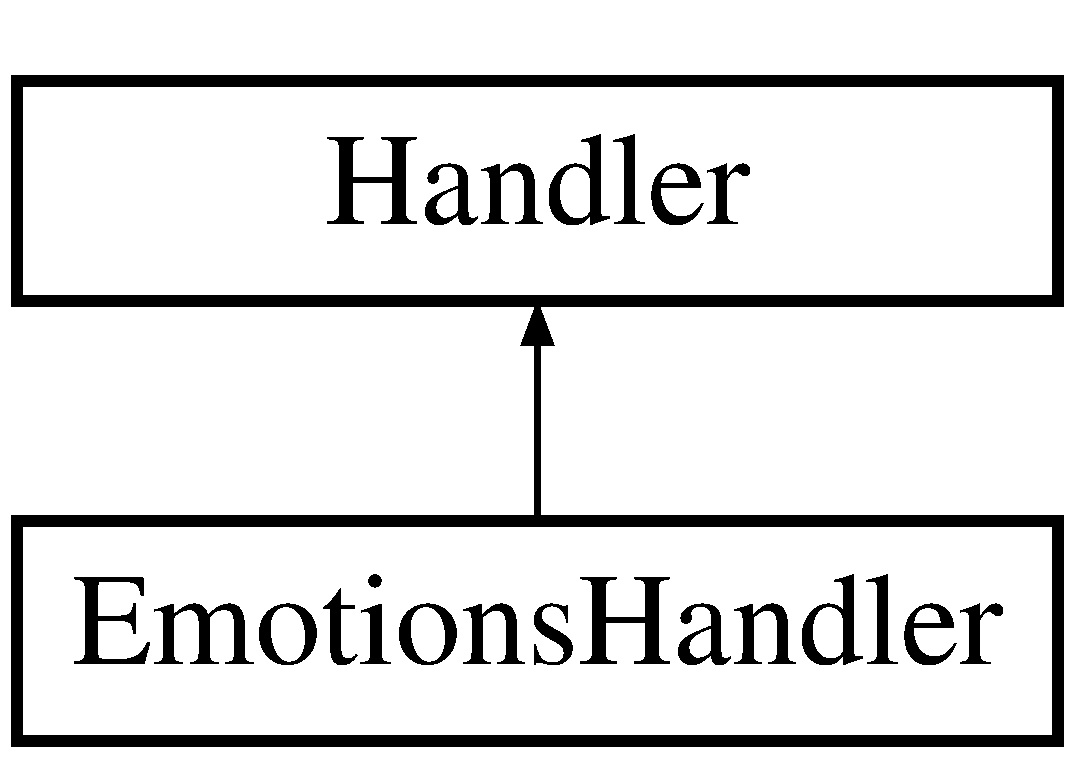
\includegraphics[height=2.000000cm]{class_emotions_handler}
\end{center}
\end{figure}
\subsection*{Public Member Functions}
\begin{DoxyCompactItemize}
\item 
\mbox{\Hypertarget{class_emotions_handler_a170b451fad0b9b50f644181de23f91f3}\label{class_emotions_handler_a170b451fad0b9b50f644181de23f91f3}} 
{\bfseries Emotions\+Handler} (\hyperlink{class_emotions_tracker}{Emotions\+Tracker} $\ast$etr)
\item 
\mbox{\Hypertarget{class_emotions_handler_afa6e3c01919c831d6b76e4848aef9742}\label{class_emotions_handler_afa6e3c01919c831d6b76e4848aef9742}} 
virtual pxc\+Status P\+X\+C\+A\+PI {\bfseries On\+New\+Sample} (pxc\+U\+ID, P\+X\+C\+Capture\+::\+Sample $\ast$sample)
\end{DoxyCompactItemize}


\subsection{Detailed Description}
Class for providing the camera event handler 

The documentation for this class was generated from the following files\+:\begin{DoxyCompactItemize}
\item 
library/emotracker/emotracker/emotracker.\+h\item 
library/emotracker/emotracker/emotracker.\+cpp\end{DoxyCompactItemize}

\hypertarget{class_emotions_tracker}{}\section{Emotions\+Tracker Class Reference}
\label{class_emotions_tracker}\index{Emotions\+Tracker@{Emotions\+Tracker}}


Class for providing the driver to process data from camera  




{\ttfamily \#include $<$emotracker.\+h$>$}

\subsection*{Public Member Functions}
\begin{DoxyCompactItemize}
\item 
\mbox{\Hypertarget{class_emotions_tracker_afb06d6882dd40a40b94ce3579769ae2c}\label{class_emotions_tracker_afb06d6882dd40a40b94ce3579769ae2c}} 
\hyperlink{class_emotions_tracker_afb06d6882dd40a40b94ce3579769ae2c}{Emotions\+Tracker} ()
\begin{DoxyCompactList}\small\item\em Constructor \end{DoxyCompactList}\item 
\mbox{\Hypertarget{class_emotions_tracker_ab4cf40eb06b6b4728053bb6d143821df}\label{class_emotions_tracker_ab4cf40eb06b6b4728053bb6d143821df}} 
\hyperlink{class_emotions_tracker_ab4cf40eb06b6b4728053bb6d143821df}{$\sim$\+Emotions\+Tracker} ()
\begin{DoxyCompactList}\small\item\em Destructor \end{DoxyCompactList}\item 
\hyperlink{class_emotions_tracker_a3fe760d853d9f56830ad241cfea10aeb}{Emotions\+Tracker} (P\+X\+C\+Sense\+Manager $\ast$m\+\_\+sm)
\begin{DoxyCompactList}\small\item\em Constructor with \end{DoxyCompactList}\item 
\mbox{\Hypertarget{class_emotions_tracker_a83fa504b5116e572602868df1cd77f6f}\label{class_emotions_tracker_a83fa504b5116e572602868df1cd77f6f}} 
pxc\+Status \hyperlink{class_emotions_tracker_a83fa504b5116e572602868df1cd77f6f}{Init} ()
\begin{DoxyCompactList}\small\item\em Initialize driver \end{DoxyCompactList}\item 
\mbox{\Hypertarget{class_emotions_tracker_a80001215d863892367d69fe4325fb41b}\label{class_emotions_tracker_a80001215d863892367d69fe4325fb41b}} 
pxc\+Status \hyperlink{class_emotions_tracker_a80001215d863892367d69fe4325fb41b}{Process\+Frame} ()
\begin{DoxyCompactList}\small\item\em Process captured frame \end{DoxyCompactList}\item 
pxc\+Status \hyperlink{class_emotions_tracker_ae0ab90b095ae541d2129b0d470f7d7ff}{Process\+Sample} (P\+X\+C\+Capture\+::\+Sample $\ast$sample)
\begin{DoxyCompactList}\small\item\em Process frame sample \end{DoxyCompactList}\item 
\mbox{\Hypertarget{class_emotions_tracker_a7a83b4e6d753fd13d541afde8d550783}\label{class_emotions_tracker_a7a83b4e6d753fd13d541afde8d550783}} 
pxc\+Status \hyperlink{class_emotions_tracker_a7a83b4e6d753fd13d541afde8d550783}{Set\+Output\+U\+RL} (pxc\+C\+H\+AR $\ast$url)
\begin{DoxyCompactList}\small\item\em Set U\+RL to write ttml output \end{DoxyCompactList}\item 
\mbox{\Hypertarget{class_emotions_tracker_a0ce7070b0331662358fcefde44b22441}\label{class_emotions_tracker_a0ce7070b0331662358fcefde44b22441}} 
\hyperlink{class_emotions_configuration}{Emotions\+Configuration} $\ast$ \hyperlink{class_emotions_tracker_a0ce7070b0331662358fcefde44b22441}{Query\+Configuration} ()
\begin{DoxyCompactList}\small\item\em Get emotions configuration class instance \end{DoxyCompactList}\item 
\mbox{\Hypertarget{class_emotions_tracker_a097d4ff8db0b4ca330bec36e2343ff73}\label{class_emotions_tracker_a097d4ff8db0b4ca330bec36e2343ff73}} 
\hyperlink{class_emotions_data}{Emotions\+Data} $\ast$ \hyperlink{class_emotions_tracker_a097d4ff8db0b4ca330bec36e2343ff73}{Query\+Output} ()
\begin{DoxyCompactList}\small\item\em Get curently collected emotions data \end{DoxyCompactList}\item 
\mbox{\Hypertarget{class_emotions_tracker_a054e0ccebc638d54b6deb1ec60f660e3}\label{class_emotions_tracker_a054e0ccebc638d54b6deb1ec60f660e3}} 
pxc\+Status \hyperlink{class_emotions_tracker_a054e0ccebc638d54b6deb1ec60f660e3}{Start} ()
\begin{DoxyCompactList}\small\item\em Start processing camera stream \end{DoxyCompactList}\item 
\mbox{\Hypertarget{class_emotions_tracker_a7b78dbd1a9ddc028b2c7ada76d5c42e5}\label{class_emotions_tracker_a7b78dbd1a9ddc028b2c7ada76d5c42e5}} 
pxc\+Status \hyperlink{class_emotions_tracker_a7b78dbd1a9ddc028b2c7ada76d5c42e5}{Stop} ()
\begin{DoxyCompactList}\small\item\em Stop processing camera stream \end{DoxyCompactList}\item 
\mbox{\Hypertarget{class_emotions_tracker_adf4a570762e9f01338acbfd9f41ce1b6}\label{class_emotions_tracker_adf4a570762e9f01338acbfd9f41ce1b6}} 
pxc\+Status \hyperlink{class_emotions_tracker_adf4a570762e9f01338acbfd9f41ce1b6}{Release} ()
\begin{DoxyCompactList}\small\item\em Release used memory \end{DoxyCompactList}\item 
\mbox{\Hypertarget{class_emotions_tracker_a49efddf4954f06dd0c1b78bc84a7f12d}\label{class_emotions_tracker_a49efddf4954f06dd0c1b78bc84a7f12d}} 
void \hyperlink{class_emotions_tracker_a49efddf4954f06dd0c1b78bc84a7f12d}{Process} ()
\begin{DoxyCompactList}\small\item\em Process camera stream \end{DoxyCompactList}\end{DoxyCompactItemize}


\subsection{Detailed Description}
Class for providing the driver to process data from camera 

\subsection{Constructor \& Destructor Documentation}
\mbox{\Hypertarget{class_emotions_tracker_a3fe760d853d9f56830ad241cfea10aeb}\label{class_emotions_tracker_a3fe760d853d9f56830ad241cfea10aeb}} 
\index{Emotions\+Tracker@{Emotions\+Tracker}!Emotions\+Tracker@{Emotions\+Tracker}}
\index{Emotions\+Tracker@{Emotions\+Tracker}!Emotions\+Tracker@{Emotions\+Tracker}}
\subsubsection{\texorpdfstring{Emotions\+Tracker()}{EmotionsTracker()}}
{\footnotesize\ttfamily Emotions\+Tracker\+::\+Emotions\+Tracker (\begin{DoxyParamCaption}\item[{P\+X\+C\+Sense\+Manager $\ast$}]{m\+\_\+sm }\end{DoxyParamCaption})}



Constructor with 


\begin{DoxyParams}{Parameters}
{\em m\+\_\+sm} & Provides ability to setup initial sense manager\\
\hline
\end{DoxyParams}


\subsection{Member Function Documentation}
\mbox{\Hypertarget{class_emotions_tracker_ae0ab90b095ae541d2129b0d470f7d7ff}\label{class_emotions_tracker_ae0ab90b095ae541d2129b0d470f7d7ff}} 
\index{Emotions\+Tracker@{Emotions\+Tracker}!Process\+Sample@{Process\+Sample}}
\index{Process\+Sample@{Process\+Sample}!Emotions\+Tracker@{Emotions\+Tracker}}
\subsubsection{\texorpdfstring{Process\+Sample()}{ProcessSample()}}
{\footnotesize\ttfamily pxc\+Status Emotions\+Tracker\+::\+Process\+Sample (\begin{DoxyParamCaption}\item[{P\+X\+C\+Capture\+::\+Sample $\ast$}]{sample }\end{DoxyParamCaption})}



Process frame sample 


\begin{DoxyParams}{Parameters}
{\em sample} & Captured sample\\
\hline
\end{DoxyParams}


The documentation for this class was generated from the following files\+:\begin{DoxyCompactItemize}
\item 
library/emotracker/emotracker/emotracker.\+h\item 
library/emotracker/emotracker/emotracker.\+cpp\end{DoxyCompactItemize}

%--- End generated contents ---

% Index
\backmatter
\newpage
\phantomsection
\clearemptydoublepage
\addcontentsline{toc}{chapter}{Index}
\printindex

\end{document}
